\chapter{Control Theory (linear, deterministic)}
\label{ch-control-th}

This chapter is
based on Ref.\cite{wikibooks-control-systems}
and \cite{wiki-signal-flow}.

We will assume that
the reader has read Section \ref{sec-laplace-trans}
on Laplace Transforms
and Section \ref{sec-z-transform}
on Z-transforms.

Control Theory (CT)
studies the optimal
control of systems
with feedback. 
The systems studied can
be 
\begin{itemize}
\item linear or non-linear,
\item deterministic or stochastic,
\item continuous time (analog)
or
discrete time (digital).
\end{itemize}
This chapter will deal
with linear deterministic
systems of either 
the analog or digital kind.

As explained in Chapter
\ref{ch-dyn-bnet},
dynamical bnets and feedback
are two ways
of viewing the same 
physical phenomenon.
Also, there are numerous examples
of dynamical bnets in this book:
Kalman filters, Hidden Markov Models,
Reinforcement Learning,
Recursive Neural Nets, to name a few.
Hence, a chapter 
on CT is very 
pertinent to this book.

Two acronyms
commonly 
used in CT books
are:
{\bf SISO} (single input single output)
and
{\bf MIMO} (multiple input multiple output). We will consider both
SISO and MIMO systems in this chapter.

Another distinction
commonly
made in CT books
is between {\bf time-variant}
and {\bf time-invariant } systems.
We will explain what those terms
mean later on in this chapter.
This chapter will consider
both types of systems.



\section{Basic feedback model}

CT uses feedback to
control
a {\bf system or process}.
Fig.\ref{fig-basic-feedback}
shows a very basic
feedback model,
represented
with 3 equivalent
diagrams.


\begin{figure}[h!]
$$
\begin{array}{ccc}
\xymatrix{
\ar[d]^{r(t)}
\\
*+[F]{\stackrel{\rm Controller}{F_1}}
\ar@{-}[d]^{u(t)}
&
\ar@{-}[d]\ar@{-}[l]
&
\\
*+[F]{\stackrel{\rm Prossess} {F_2}}
\ar@{-}[r]^{\quad y(t)}
&\ar@{-}[u]
}
&
\xymatrix{
\rvr^{[k]}\ar[d]
&
\rvr^{[k+1]}\ar[d]
\\
\rvu^{[k]}\ar[d]
&\rvu^{[k+1]}\ar[d]
\\
\rvy^{[k]}\ar[r]\ar[ur]
&
\rvy^{[k+1]}
}
&\quad\quad
\xymatrix{
\rvr(t)\ar[d]
\\
\rvu(t)\ar[d]
\\
\rvy(t)
\ar@(ul,ur)@{~>}[]
\ar@{~>}@/_2pc/[u]
}
\\
\\
(a)&(b)&\quad\quad(c)
\end{array}
$$
\caption{Basic feedback model
represented as: $(a)$ a
wired-boxes diagram, $(b)$ one
slice of a dynamical bnet 
(see Chapter \ref{ch-dyn-bnet}),
and $(c)$ a ``rolled" dynamical bnet
 with feedback cycles. 
}
\label{fig-basic-feedback}
\end{figure}

The diagrams of 
Fig.\ref{fig-basic-feedback}
represent
graphically
the following
system
of equations.
Here $t\in[0,\infty]$
is time and
$u,y:[0,\infty]$.

\beq
\left\{
\begin{array}{l}
u(t) = F_1(y(t), r(t), t)
\\
\partial_t y(t)= F_2(y(t), u(t), t)
\end{array}
\right.
\eeq
If we approximate the 
time derivative of $y(t)$ by

\beq
\partial_t y(t) \approx 
\frac{y(t+
\Delta t)-y(t)}{\Delta t}
\eeq
and we set

$t_k=t$, $t_{k+1}=t + \Delta t$, $0< \Delta t<< 0$, 

$f(t_k)=f^{[k]}$ for $f=y,u$,
\\then we get 
Fig.\ref{fig-basic-feedback}

The TPMs, 
printed in blue,
of the bnet
in Fig.\ref{fig-basic-feedback},
are as follows:

\beq \color{blue}
P(r^{[k]}) = \text{given}
\eeq

\beq\color{blue}
P(u^{[k]}|y^{[k]}, r^{[k]}) = 
\delta(\quad
u^{[k]}- F_1(y^{[k]}, r^{[k]}, t_k)
\quad)
\eeq


\beq\color{blue}
P(y^{[k+1]}|y^{[k]}, u^{[k]})
=
\delta(\quad
y^{[k+1]}
- y^{[k]} -\Delta t F_2(y^{[k]}, u^{[k]}, t_k)
\quad)
\eeq




\section{Classical model (analog)}


\begin{figure}[h!]
$$
\begin{array}{ccc}
\xymatrix{
\ar[d]_{r(t)}^{+}
\\
*+[F]{\sum}
\ar@{-}[d]_{e(t)}
&\ar@{-}[l]^{-}_{f(t)}
\\
*+[F]{\stackrel{\rm Controller}{C}}
\ar@{-}[d]_{u(t)}
&
*+[F]{\stackrel{\rm Filter} {F}}
\ar@{-}[u]\ar@{-}[d]
&
\\
*+[F]{\stackrel{\rm Prossess} {\Pi}}
\ar@{-}[r]^{y(t)}
\ar[d]^{y(t)}
&\ar@{-}[u]
\\
&
}
&
\xymatrix@C=3pc{
\rvf^{[k]}\ar@/_1.5pc/[dd]
&
\rvf^{[k+1]}\ar@/_1.5pc/[dd]
\\
\rvr^{[k]}\ar[d]
&
\rvr^{[k+1]}\ar[d]
\\
\rve^{[k]}\ar[d]\ar[rd]
&
\rve^{[k+1]}\ar[d]
\\
\rvu^{[k]}\ar[d]\ar[rd]
&\rvu^{[k+1]}\ar[d]
\\
\rvy^{[k]}\ar[ruuuu]
&
\rvy^{[k+1]}
}
&\quad\quad
\xymatrix{
\rvf(t)\ar@/_1.5pc/[dd]
\\
\rvr(t)\ar[d]
\\
\rve(t)\ar[d]\ar@{~>}@/_1pc/[d]
\\
\rvu(t)\ar[d]\ar@{~>}@/_1pc/[d]
\\
\rvy(t)\ar@{~>}@/_2pc/[uuuu]
}
\\
\\
(a)& (b) &\quad\quad (c)
\end{array}
$$
\caption{
Classical Model
represented
with
the same 3
types of diagrams
as Fig.\ref{fig-basic-feedback}.
Bnets $(b)$ and $(c)$
don't
show all the arrows.
In reality,
for any arrow $a^{[k]}\rarrow b^{[k+1]}$ that
points from the 
time slice $t_k$
to the time slice $t_{k+1}$,
there should 
be arrows 
$a^{[j]}\rarrow b^{[k+1]}$
for $j\in\{0,1,2, \cdots, k
\}$.
That's because
the classical model is defined
in terms of convolutions,
and a convolution
at time $t$ requires
memory for all times
between 0 and $t$.
If we take
the Laplace transform
of figures $(a)$ and $(c)$ (or 
the Z-transform of figure $(b)$),
then we get a
Signal Flow (SF) graph. SF graphs will
be discussed later on in this chapter.
In SF graphs,
the only
inter slice arrows are between 
adjacent slices; i.e., SF graphs have
no arrows that 
span more than 1 slice.}
\label{fig-classic-model}
\end{figure}
A {\bf classical
model} is a bunch of
 convolution boxes
 connected by wires.
 See Fig.\ref{fig-classic-model}
 for 3
 graphical
 representations of
 the classical model.
 
The diagrams of 
Fig.\ref{fig-classic-model}
represent
graphically
the following
system
of equations.
Here $t\in[0,\infty]$
is time and
$f,e,u,y:[0,\infty]\rarrow \CC$.

\beq
\left\{
\begin{array}{l}
f(t) = (F\circledast  y)(t)
\\
e(t)= r(t) - f(t)
\\
u(t) = (C\circledast  e)(t)
\\
y(t) = (\Pi\circledast  u)(t)
\end{array}
\right.
\label{eq-classic-analog}
\eeq
where $()f\circledast g)(t)$
denotes a covolution,
as defined in Section \ref{sec-laplace-trans}
on Laplace transforms.

The TPMs, 
printed in blue,
of the bnet
in Fig.\ref{fig-classic-model},
are as follows:

\beq\color{blue}
P(r(t)) = \text{given}
\eeq

\beq\color{blue}
P(f(t)|y(\cdot))
=\delta(\quad
f(t)-\Pi[y](t)
\quad)
\eeq

\beq\color{blue}
P(e(t)|
r(t), f(t))=
\delta(\quad
e(t)- [r(t)-f(t)]
\quad)
\eeq

\beq\color{blue}
P(u(t)|e(\cdot))=
\delta(\quad
u(t)-C[e](t)
\quad)
\eeq

\beq\color{blue}
P(y(t)|u(\cdot))
=\delta(\quad
y(t)-\Pi[u](t)
\quad)
\eeq


If we take
the Laplace transform
of Eqs.(\ref{eq-classic-analog},
we get

\beq
\left\{
\begin{array}{l}
\TIL{f}(s) =\TIL{F}(s)\TIL{y}(s)
\\
\TIL{e}(s)= \TIL{r}(s) - \TIL{f}(s)
\\
\TIL{u}(s) = \TIL{C}(s)\TIL{e}(s)
\\
\TIL{y}(s) = \TIL{\Pi}(s)\TIL{u}(s)
\label{eq-classic-analog-lap}
\end{array}
\right.
\eeq
Thus

\beq
\TIL{y}=\TIL{\Pi}\TIL{C}[\TIL{r}-
\TIL{F}\TIL{y}]
\eeq

\beq
[1+\TIL{\Pi}\TIL{C}\TIL{F}]\TIL{y}
=
\TIL{\Pi}\TIL{C}\TIL{r}
\eeq
From this,
we can solve for the 
{\bf transfer or gain function}
$\TIL{H}_{y|r}(s)$

\beqa
\TIL{H}_{y|r}(s)
&=&
\frac{\TIL{y}(s)}{\TIL{r}(s)}
\quad \text{(output/input)}
\\
&=&
\frac{
\overbrace{\TIL{\Pi}\TIL{C}}^{
H_0=
\TIL{H} \text{ with } F=0}
}
{1 + 
\underbrace{\TIL{\Pi}\TIL{C}\TIL{F}
}_{H_0\TIL{F}}
}
\eeqa

A special
and very common
type of controller
function $u(t)$
called the 
{\bf Proportional-Integral-Derivative (PID) Controller}
is defined as

\beq
u(t)=
K_\Pi e(t)
+K_I
\int_0^t
d\tau \;
e(\tau)
+
K_D\partial_t e(t)
\eeq
The Laplace transform
of the PID controller
is 


\beqa
\TIL{u}(s)
&=&
K_\Pi\TIL{e}(s)
+ K_I \frac{\TIL{e}}{s}
+
K_D (s\TIL{e}(s)-
e(0^+))
\\
&=&
\underbrace{
\left(
K_\Pi + \frac{K_I}{s}
+ K_D s
\right)
}_{\TIL{C}(s)}
\TIL{e}(s)
\quad\text{(assume $e(0^+)=0$)}
\eeqa


\begin{claim}
A PID controller
has unit gain ($\TIL{H}_{y|r}(s)=1$)
if its
defining parameters satisfy:

\beq
K_\Pi = 2K,\;
K_D=KT,\; K=\frac{K}{T}
\eeq
\end{claim}
\proof

\beq
\TIL{\Pi}(s)= \frac{1}{K(1+sT)}
\eeq
and

\beq
\TIL{F}(s) = \frac{1}{1+sT}
\eeq
so


\beqa
\TIL{C}
&=&\frac{K}{sT}\left(2sT +1 + (sT)^2\right)
\\
&=&
\frac{K}{sT}\left(1 +sT\right)^2
\eeqa
and

\beqa
1+\TIL{\Pi}\TIL{C}\TIL{F}&=&
1+\frac{1}{sT}
\\
&=&\frac{1}{sT}(1+sT)
\\
&=&
\TIL{\Pi}\TIL{C}
\eeqa
Hence,

\beq
\TIL{H}_{y|r}(s)=1
\quad \text{(output/input)}
\eeq
\qed






\section{Modern model (analog) }


 \begin{figure}[h!]
 $$
\begin{array}{ccc}
\xymatrix@R=2pc{
\ar[d]^{u(t)}
\\
\ar@/_2pc/@{-}[dd]_{u(t)}
\ar@{-}[d]^<<<{u(t)}
\\
*+[F]{F_{AB}}
\ar@{-}[d]^{x(t)}
\ar@(ul,ur)@{-}[]
\\
*+[F]{F_{CD}}
\ar[d]^{y(t)}
\\
&
}
&
\xymatrix@C=4pc{
\rvu^{[k]}\ar@/_2pc/[dd]_D
\ar[rd]^<<<{B}
& \rvu^{[k+1]}\ar@/_2pc/[dd]
\\
\rvx^{[k]}\ar[d]_C\ar[r]^<<<{A}
&\rvx^{[k+1]}\ar[d]
\\
\rvy^{[k]}
&\rvy^{[k+1]}
}
&\quad\quad
\xymatrix{
\rvu(t)\ar@/_2pc/[dd]
\ar@{~>}[d]
\\
\rvx(t)\ar[d]
\ar@(ul,ur)@{~>}[]
\\
\rvy(t)
}
\\
\\
(a)&(b)&\quad\quad(c)
\end{array}
$$
\caption{Modern Model
represented
with
the same 3
types of diagrams
as Fig.\ref{fig-basic-feedback}.}
\label{fig-modern-model}
\end{figure}

A {\bf modern
model (a.k.a. state space model)} is a bunch of
 time dependent
 boxes, some with 
 first order
 time derivatives, 
 connected by wires.
 See Fig.\ref{fig-modern-model}
 for 3
 graphical
 representations of
 the classical model.

The diagrams of 
Fig.\ref{fig-modern-model}
represent
graphically
the following
system
of equations.
Here $t\in[0,\infty]$
is time and

$u:[0, \infty]\rarrow \CC^{nu}$

$x:[0, \infty]\rarrow \CC^{nx}$

$y:[0, \infty]\rarrow \CC^{ny}$
\\ for some integers $nu, nx, ny$.
These
equations are
called the {\bf state space equations} and $x(t)$ is called the {\bf state} 
of the system.
\beq
\left\{
\begin{array}{l}
\partial_t x(t)= F_{AB}(x(t), u(t), t)
\\
y(t) = F_{CD}(x(t), u(t), t)
\end{array}
\right.
\label{eq-nonlinear-modern}
\eeq

The TPMs, 
printed in blue,
of the bnet
in Fig.\ref{fig-modern-model},
are as follows:


\beq\color{blue}
P(u^{[k]})=\text{given}
\eeq

\beq\color{blue}
P(x^{[k+1]}\cond x^{[k]}, u^{[k]})=
\delta(\quad
x^{[k+1]}- \Delta t F_{AB}(x^{[k]}, u^{[k]}, t_k)
\quad)
\eeq

\beq\color{blue}
P(y^{[k+1]}\cond x^{[k]}, u^{[k]})
=
\delta(\quad
y^{[k+1]}-F_{CD}(x^{[k+1]},
u^{[k+1]}, t_{k+1})
\quad)
\eeq




Henceforth, assume $F_{AB}$
and $F_{CD}$ are as follows. This is called
the {\bf linear} case.

\beq
\left\{
\begin{array}{l}
F_{AB}(x(t), u(t)) = A(t)x(t) + B(t)u(t)
\\
F_{CD}(x(t), u(t)) = C(t)x(t) + D(t)u(t)
\end{array}
\right.
\eeq
for some
matrices
$A(t), B(t), C(t), D(t)$.
In the linear case,
the modern model is
described by the following
equations:

\beq
 \left\{
 \begin{array}{l}
 \partial_t x(t) = A x(t) + B u(t)
 \\
 y(t) = C x(t) + D u(t)
 \end{array}
 \right.
 \label{eq-modern-linear-analog}
 \eeq
 
 

If the 
matrices  $A(t), B(t), C(t), D(t)$
depend on (resp., are independent of)
time $t$,
we say the system
is {\bf time-variant}
(resp., {\bf time-invariant}).
Next, we solve the 
differential
equation for
$x(t)$,
for both the time-invariant and variant cases.

\begin{itemize} 
\item time-invariant case


Taking the Laplace transform
of the first equation of
Eqs.(\ref{eq-modern-linear-analog}),
we get

\beq
s\TIL{x}(s)-x(0)=A\TIL{x}(s) + B\TIL{u}(s)
\eeq
Hence,
the Laplace transform
of Eqs.(\ref{eq-modern-linear-analog})
is
 
 \beq
 \left\{
 \begin{array}{l}
 \TIL{x}(s) = (sI-A)^{-1} x(0)
 + (sI-A)^{-1} B\TIL{u}(s)
 \\
 \TIL{y}(s)=C\TIL{x}(s)+ D\TIL{u}(s)
 \end{array}
 \right.
 \eeq

If we define the transfer function
 $\TIL{H}_{y|u}(s)$ by
  
 \beq
 \underbrace{\TIL{y}(s)}_{output}=
 \TIL{H}_{y|u}(s)
 \underbrace{\TIL{u}(s)}_{input}
 \eeq
 then,
 assuming $x(0)=0$,
  
 \beq
 \TIL{H}_{y|u}(s) =
 C(sI-A)^{-1}B
 +D
 \eeq
  
 
 \begin{claim}
 \beq
 x(t)=e^{A(t-t_0)}x(t_0)
 +
 e^{A(t-t_0)}
 \int_{t_0}^{t} d\tau\;
 e^{-A(\tau-t_0)}
 Bu(\tau)
 \label{eq-state-space-sol}
 \eeq
 where
 
 \beq
 e^{At}= \sum_{k=0}^\infty
 \frac{t^k}{k!}A^k
 \eeq
 Hence, setting $t\geq t_0=0$,
 \beq
  e^{At}=
  \call^{-1}[(sI-A)^{-1}]
  \eeq
  
  \beq
  e^{At}
    \int_0^t d\tau\;
    e^{-\tau}
    Bu(\tau)
    =
   \call^{-1}[
  (sI-A)^{-1}B\TIL{u}(s)]
   \eeq
   
 \end{claim}
 \proof
 To check Eq.(\ref{eq-state-space-sol}),
 just take the time derivative
 of both sides and 
 use $\partial_t\int^t d\tau\; f(\tau)= 
 f(t)$
 \qed
 
 \item time-variant case
 
 \begin{claim}
 \label{cl-modern-time-variant}
 
 \beq
 x(t)=
 \cale(t,t{_0})x(t_0)
 +
 \int_{t_0}^t
 d\tau\;
 \cale(t,\tau)
 B(\tau)u(\tau)
 \label{eq-time-var-sol}
 \eeq
 where
 the {\bf transition matrix
 (a.k.a. evolution matrix)} $\cale(t, t_0)$
 satisfies
 
 \beq
 \partial_t 
 \cale(t, t_0) = A(t)
 \eeq
and

\beq
\cale(t,t)=1
\eeq

 \end{claim}
 \proof 
 To prove Eq.(\ref{eq-time-var-sol}),
 just differentiate both sides of it
 with respect to $t$,
 and use $\partial_t\int^td\tau\; f(\tau) = f(t)$
 \qed
 
 In the time-invariant case,
 
 \beq 
 \cale(t,t_0)=e^{A(t-t_0)}
 \eeq
 
 
 
 \end{itemize}
 
 \section{Classical model (digital)} 
 In this section,
 we will define
 the classical model
 with discrete rather
 than continuous time.
 
 If we discretize time (i.e., 
 sample time
 at discrete times
 separated by a time
 interval $T$),
 then 
 the equivalent 
 of Eqs.(\ref{eq-classic-analog})
 is
 
 \beq
 \left\{
 \begin{array}{l}
 f^{[n]} = (F\circledast  y)^{[n]}
 \\
 e^{[n]}= r^{[n]} - f^{[n]}
 \\
 u^{[n]} = (C\circledast  e)^{[n]}
 \\
 y^{[n]} = (\Pi\circledast  u)^{[n]}
 \end{array}
 \right.
 \label{eq-classic-digital}
 \eeq
 where $(x\circledast y)^{[n]}$
denotes a 
discrete convolution, as 
defined in Section
 \ref{sec-z-transform}
 on Z-transforms.
 And
 if we take
 the Z-transform
 of Eqs.(\ref{eq-classic-digital}),
 we get
 
 \beq
 \left\{
 \begin{array}{l}
 \TIL{f}(z) =\TIL{F}(z)\TIL{y}(z)
 \\
 \TIL{e}(z)= \TIL{r}(z) - \TIL{f}(z)
 \\
 \TIL{u}(z) = \TIL{C}(z)\TIL{e}(z)
 \\
 \TIL{y}(z) = \TIL{\Pi}(z)\TIL{u}(z)
 \end{array}
 \right.
 \eeq
 
 
 
 \section{Modern model (digital)}
 
 In this section,
  we will define
  the modern model
  with discrete rather
  than continuous time.
We will do this
2 different ways. 
First, we will 
approximate the time derivates
in a differential equation
with a discrete approximation.
This approach is interesting
and instructive but
not perfect, because
it's an approximation.
Second, we will define
difference equations
and solve them exactly.
The second approach 
is better for most purposes,
because it gives exact results,
not approximations.
 
 
 \subsection{Discretizing analog model}
 
 
  
 Ibf we approximate
 $\partial_t x(t)$ by
 
 \beq
 \partial_t x(t)=
 \lim_{\Delta t\rarrow 0}
 \frac{x(t+\Delta t)-x(t)}{\Delta t}
 \eeq
 then Eqs.(\ref{eq-modern-linear-analog})
 reduce to
 
 \beq
 \left\{
 \begin{array}{l}
 x(t+\Delta t) = (1 +\Delta t A) x(t) +\Delta t B u(t)
 \\
 y(t) = C x(t) + D u(t)
 \end{array}
 \right.
 \eeq
 Using the new notation
 
 \beq
 \HAT{A} = 
 e^{A\Delta t}\approx 1+\Delta t A,
 \eeq
 
 \beq
 \HAT{B}\approx \Delta t B
 \eeq
 
 \beq
 \Delta t = T,
 \quad t = nT
 \eeq
 
 \beq
 x(t) = x(nT) = x^{[n]},
 \quad u(t) = u(nT)= u^{[n]}
 \eeq 
 we get
 
 \beq
 \left\{
 \begin{array}{l}
 x^{[n+1]} = 
 \HAT{A} x^{[n]} + \HAT{B} u^{[n]}
 \\
 y^{[n]} = C x^{[n]} + D u^{[n]}
 \end{array}
 \right.
 \label{eq-modern-difference-eqs}
 \eeq
 
 Setting
 $t=t_0+T$ in 
  Eq.(\ref{eq-state-space-sol}),
  we get
 
 \begin{align}
  x(t_0+T)&=
  e^{AT}x(t_0)
  +
  e^{AT}
  \int_{t_0}^{t_0+T} d\tau\;
  e^{-A(\tau-t_0)}
  Bu(\tau)
  \\
  &=
   e^{AT}x(t_0)
   +
   e^{AT}
   \int_{0}^{T} d\tau\;
   e^{-A\tau}
   Bu(\tau+t_0)
   \quad\text{(substitute $\tau\rarrow 
   \tau+t_0$)}
  \end{align}
  Now setting
  
  \beq
  t_0=nT
  \eeq
  and
  
  \beq
   u(\tau + t)\approx u(t)
  \quad\text{for $\tau\in [0, T]$}
  \eeq
  we get
  
  \beq
  x^{[n+1]}=
  \underbrace{e^{AT}}_{\HAT{A}}
  x^{[n]}
    +
    \underbrace{
    e^{AT}
    \left[
    \int_{0}^{T} d\tau\;
    e^{-A\tau}
    \right]
    B}_{\HAT{B}}
    \;u^{[n]}
 \eeq
 where
 
 \beq
 \HAT{A}=e^{AT}
 \eeq
 and
 
 \beqa
 \HAT{B}
 &=&
 e^{AT}
    \left[
    \int_{0}^{T} d\tau\;
    e^{-A\tau}
    \right]
    B
 \\
 &=&
 e^{AT}(-A)^{-1}(e^{-AT}-I)B
 \\
 &=&
 A^{-1}
 (\HAT{A}-1)B
 \eeqa
 When $T<<1$,
 $\HAT{A}-1\approx AT$
 so $A^{-1}
 (\HAT{A}-1)B\approx BT$.
 
 \subsection{Solving Difference Equation}
 
 \begin{itemize}
 \item time-invariant case
 
 Consider the following difference equation
 taken from
 Eqs.(\ref{eq-modern-difference-eqs})
 
 \beqa
 x^{[n+1]} &=& \HAT{A}x^{[n]}+\HAT{B}u^{[n]}
 \eeqa
 To solve
 this difference equation,
 we notice that
 
 
 \beqa
  x^{[1]} &=& \HAT{A}x^{[0]}+
  \HAT{B}u^{[0]}
  \eeqa
  
\beqa
x^{[2]}&=& \HAT{A}x^{[1]}
+\HAT{B}u^{[1]}
\\
&=&
\HAT{A}^2 x^{[0]}
+\HAT{A}\HAT{B}u^{[0]}
++\HAT{B}u^{[1]}
\eeqa
 
 \beqa
 x^{[2]}&=&\HAT{A}x^{[2]}+ \HAT{B}u^{[2]}
 \\
 &=&
 \HAT{A}^3 x^{[0]}
 + \HAT{A}^2 \HAT{B}u^{[0]}
 + \HAT{A}\HAT{B} u^{[1]}
 + \HAT{B} u^{[2]}
 \eeqa
 The general pattern is clear.
 In general,  
 
 \beq
 x^{[n]}=
 \HAT{A}^n x^{[n_0]}
 +\sum_{k=0}^{n-1}
 \HAT{A}^{n-k-1}
 \HAT{B} u^{[k]}
\eeq

It is also possible
to solve Eqs.(\ref{eq-modern-difference-eqs})
using Z-transforms (See Section
\ref{sec-z-transform}).
The Z-transform
of the first of
those two equations is

\beq
z(\TIL{x}(z) - x^{[0]})
= \HAT{A}\TIL{x}(z) + \HAT{B}\TIL{u}(z)
\eeq
Therefore, the
Z-transform of 
Eqs.(\ref{eq-modern-difference-eqs}) is\footnote{Notice the
$z$ factor multipying
$x^{[0]}$. There 
is no counterpart $s$
factor
multiplying $x(0)$
in the analog case.
That's because $z=e^{sT}$.}

\beq
\left\{
\begin{array}{l}
\TIL{x}(z) = (zI -\HAT{A})^{-1}z x^{[0]}
+
(zI -\HAT{A})^{-1}\HAT{B}\TIL{u}(z)
\\
\TIL{y}(z)= C\TIL{x}(z) + D\TIL{u}(z)
\end{array}
\right.
\eeq
From this
we can get the transfer matrix $\TIL{H}_{y|u}(z)$. Assuming $x^{[0]}=0$, 

\beq
\TIL{y}(z)=
\underbrace{
\left(
\HAT{C}(zI-\HAT{A})^{-1}\HAT{B}
+\HAT{D}
\right)}_{\TIL{H}_{y|u}(z)}
\TIL{u}(z)
\eeq


 
 \item time-variant case
 
 We can also give a
 discrete version of Claim
 \ref{cl-modern-time-variant}
 
 \begin{claim}
  \beq
  x^{[n]}=
  \cale^{[n,n_0]}x^{[n_0]}
  +\sum_{k=0}^{n-1}
  \cale^{[n, k+1]}
  B^{[k]} u^{[k]}
 \eeq
 where
 
 \beq
 \cale^{[n+1, n_0]}=\HAT{A}^{[n]}
 \cale^{[n,n_0]}
 \eeq
 and
 
 \beq
 \cale^{[n_0, n_0]} = I
 \eeq
 Hence
 
 \beqa
 \cale^{[n,n_0]}&=&
 \HAT{A}^{[n-1]}\HAT{A}^{[n-2]}
 \HAT{A}^{[n-3]}\cdots \HAT{A}^{[n_0]}
 \\
 &=&
 \prod_{k\in \ZZ^{[1, n-n_0]}}\HAT{A}^{[n-k]}
 \eeqa
 \end{claim}
 \proof Left to reader.
 \qed
 
 \end{itemize}
 
 
  \section{Higher than first order differential (or difference) equations}
  
If in the time-invariant
analog modern model, 
we express $x(t)$
in terms of $y(t)$
and $u(t)$

\beq
x(t)= C^{-1}[y(t) -Du(t)]
\eeq
and then we plug this into the
equation for $\partial_t x(t)$,
we get

\beq
\partial_t
\left(
\underbrace{
 C^{-1}[y(t) -Du(t)]}_{x(t)}
\right)
= A \underbrace{
 C^{-1}[y(t) -Du(t)]}_{x(t)} + Bu(t)
\eeq
Hence, it appears
that this model can
only accommodate a
first order time derivative
of the output $y(t)$.
Next we give
a transformation 
whereby a model
with
$y(t)$ derivatives that are higher
than 1st order,
can be re-expressed
in a form
that only 
has 1st order
time derivatives.
We will
also give
an analogous result for 
the time-invariant digital modern
model. We will show that those  
digital models 
can accommodate higher
than 1st order 
time differences.
  
  \subsection{Differential Equations}
 Let
 \beq
 \Omega = \partial_t^3
 + a_2\partial_t^2 + a_1\partial_t + a_0
 \eeq
 where $a_0, a_1, a_2\in \CC$ are 
 independent of time $t$,
 and consider the {\bf linear,
 constant
 coefficients (LCC) ordinary differential
 equation (ODE)}:
 
 \beq
 \Omega y(t)= u(t)
 \eeq
 Assume $f(t)$ satisfies
 
 \beq
 \Omega f(t)=0
 \eeq
Let

\beq
\underbrace{\partial_t^3 y(t)}_{
\partial_t x_2+\partial_t^3 f}
+ a_2\underbrace{\partial_t^2 y(t)}_{x_2
+\partial_t^2 f}
+ a_1 \underbrace{\partial_t y(t)}
_{x_1+\partial_t f}
+ a_0 \underbrace{y(t)}_{x_0+f}
 =u(t)
\eeq

\beq
x(t)=
\left[
\begin{array}{c}
x_0(t)
\\
x_1(t)
\\
x_2(t)
\end{array}
\right]
\eeq
Then

\beq
\partial_t x(t)=
\underbrace{\left[
\begin{array}{ccc}
0&1&0
\\
0&0&1
\\
-a_0&-a_1&-a_2
\end{array}
\right]
}_{A}
x(t)
+ \underbrace{\left[
\begin{array}{c}
0
\\
0
\\
1
\end{array}
\right]}_{B}
u(t)
\eeq

\beq
y(t) = x_0(t) + f(t)=
\underbrace{\left[
\begin{array}{ccc}
1&0&0
\end{array}
\right]
}_{C}
x(t)
+ f(t)
\eeq
If $\Omega u=0$, we can define $f=D u$.
Otherwise, define $f=0$.

What's going on here, from 
a dynamical bnet perspective,
is that we are defining the slices 
to have enough variables 
so that there only needs to be
memory from one slice to the previous 
slice instead of to the
previous 3 slices.

\subsection{Difference Equations}
Let 

\beq
\underbrace{y^{[n+3]}}_{x_3^{[n+1]}}
+ a_2 \underbrace{y^{[n+2]}}_{x_2^{[n]}}
+ a_1 \underbrace{y^{[n+1]}}_{x_1^{[n]}}
+ a_0 \underbrace{y^{[n]}}_{x_0^{[n]}}
=
u^{[n]}
\eeq
Then

\beq
x^{[n]}=
\left[
\begin{array}{c}
x_0^{[n]}
\\
x_1^{[n]}
\\
x_2^{[n]}
\end{array}
\right]
\eeq

\beq
x^{[n+1]}=
\underbrace{\left[
\begin{array}{ccc}
0&1&0
\\
0&0&1
\\
-a_0&-a_1&-a_2
\end{array}
\right]
}_{A}
x^{[n]}
+ \underbrace{\left[
\begin{array}{c}
0
\\
0
\\
1
\end{array}
\right]}_{B}
u^{[n]}
\eeq

\beq
y^{[n]} = x_0^{[n]}=
\underbrace{\left[
\begin{array}{ccc}
1&0&0
\end{array}
\right]
}_{C}
x^{[n]}
\eeq



\section{Causality, Stability, Controlability, Observability}

Suppose $x, u, y:\calt\rarrow \calx$.
 where $\calt=[0, \infty)$.

\subsection{Causality, Stability}


 

$y(\cdot)$ is {\bf stable}
if $x(\cdot)$ 
and $u(\cdot)$ bounded implies
$y(\cdot)$ is bounded.


\subsection{
Controllability,
Observability}
$a\in\calx$ is {\bf controllable
(resp., reachable) at time $t_0\in\calt$
}
if there exist a time
$t_1\in\calt$ and an input $u(\cdot)$ such that $x(t_0)=a$
and $x(t_1)=0$ (resp., $x(t_0)=0$ and $x(t_1)=a$)
$x(\cdot)$ is {\bf controllable 
(resp., reachable)
at time $t_0\in\calt$}
if it is controllable 
(resp., reachable)
at time $t_0\in\calt$ for all $a\in\calx$.


$a\in\calx$ is {\bf observable at time $t_0\in\calt$}
if there exists a $t_1\in \calt$
such that 
$x(t_0)=a$
and $a$
can be determined from
the values of 
$y(t)$ for $t\in [t_0, t_1]$.
$x(\cdot)$ is {\bf observable
at time $t_0\in\calt$ } 
if it is 
observable 
at time $t_0\in\calt$ for all $a\in \calx$.

\section{Signal Flow Graph}
This section is based on Ref.\cite{wiki-signal-flow}

Fig.\ref{fig-basic-flow-graph}
is 
the Laplace transform
of Figs.\ref{fig-classic-model} 
$(a)$ and $(c)$.
It shows 2
graphical representations 
(as a wired-boxes diagram and
as a bnet with feedback cycles) of the
Laplace transform of the
classical
model.
Note that in going 
from the wired-boxes diagram
to the bnet,
the wire labels become the node
labels,
and the box labels 
become
the arrow labels.
Note also
that node and arrow
labels are all
Laplace Transforms.



\begin{figure}[h!]
$$
\begin{array}{cc}
\xymatrix{
\ar[d]_{\TIL{r}}^{+}
\\
*+[F]{\sum}
\ar@{-}[d]_{\TIL{e}}
&\ar@{-}[l]^{-}_{\TIL{f}}
\\
*+[F]{\stackrel{\rm Controller}{\TIL{C}}}
\ar@{-}[d]_{\TIL{u}}
&
*+[F]{\stackrel{\rm Filter} {\TIL{F}}}
\ar@{-}[u]\ar@{-}[d]
&
\\
*+[F]{\stackrel{\rm Prossess} {\TIL{\Pi}}}
\ar@{-}[r]^{\TIL{y}}
\ar[d]^{\TIL{y}}
&\ar@{-}[u]
\\
&
}
&
\xymatrix{
\TIL{\rvf}\ar@/_1.5pc/[dd]_{-1}
\\
\TIL{\rvr}\ar[d]^{+1}
\\
\TIL{\rve}\ar[d]_{\TIL{C}}
\\
\TIL{\rvu}\ar[d]_{\TIL{\Pi}}
\\
\TIL{\rvy}\ar@/_2pc/[uuuu]_{\TIL{F}}
}
\end{array}
$$
\caption{This figure
is
the Laplace transform 
of Figs.\ref{fig-classic-model}
$(a)$ and
$(c)$.
}
\label{fig-basic-flow-graph}
\end{figure}

Fig.\ref{fig-basic-flow-graph}
$(c)$ is what is called a Signal
Flow (SF) graph. According
to Wikipedia Ref.\cite{wiki-signal-flow},
SF graphs were invented by Shannon
in 1942, and later 
studied and promoted by Mason.



The SF graph of Fig.\ref{fig-basic-flow-graph}
implies the following 
system of equations:

\beq
\left\{
\begin{array}{l}
\TIL{\rve}=\TIL{\rvr}-\TIL{\rvf}
\\
\TIL{\rvu}=\TIL{C}\TIL{\rve}
\\
\TIL{\rvy}=\TIL{\ul{\Pi}}\TIL{\rvu}
\\
\TIL{\rvf}=\TIL{F}\TIL{\rvy}
\end{array}
\right.
\eeq
From this system of
equations,
we find that

\beq
\TIL{y} =\TIL{\Pi}\TIL{C}
(\TIL{r}-
\underbrace{\TIL{f}}_{\TIL{F}\TIL{y}})
\eeq
Hence,
just as we found previously, the transfer function
$\TIL{H}_{y|r}(s)$ is given by

\beq
\TIL{H}_{y|r}(s)=
\frac{\TIL{y}}{\TIL{r}}
=
\frac{\TIL{\Pi}\TIL{C}}
{1+\TIL{\Pi}\TIL{C}\TIL{F}}
\eeq

SF graphs are 
the same as 
LDEN (Linear Deterministic
with External Noise) bnets discussed in
Chapter \ref{ch-linear-sys},
except for 2 important
differences: (1) SF graphs
have no external random nodes
(2)
unlike the LDEN considered in 
Chapter \ref{ch-linear-sys},
SF graphs can have feedback cycles.

In SF graphs, the
multiplicative factors
carried by the arrows  are called 
``gains".

Next, we shall discuss
some properties of the
feedback cycles of SG graphs.



An approach
that I like
is to 
re-express
an SF graph 
with feedback cycles
by one without them
that is easier to understand.

\begin{claim}
Getting rid of bubbles (i.e., self feedback cycles)
\beq
\begin{array}{ccc}
\xymatrix{
\rva\ar[dr]_{\alpha}
&
&\rvb\ar[dl]^{\beta}
\\
&\rvx\ar@(ul,ur)[]^\mu
}
&\xymatrix{\\=}&
\xymatrix{
\rva\ar[dr]_{\frac{\alpha}{1-\mu}}
&
&\rvb\ar[dl]^{\frac{\beta}{1-\mu}}
\\
&\rvx
}
\end{array}
\eeq
\end{claim}
\proof
From the left hand diagram,

\beq
\rvx=\mu\rvx + \alpha\rva + \beta\rvb
\eeq
Hence, 
\beq
\rvx =
\frac{\alpha}{1-\mu}\rva
+
\frac{\beta}{1-\mu}\rvb
\eeq
\qed

\begin{claim}
Getting rid of 2-node  cycles
\beq
\begin{array}{ccc}
\xymatrix{
\rva\ar[d]_\alpha
&\rvb\ar[d]^\beta
\\
\rvx\ar@/^1pc/[r]^\mu
&\rvy\ar@/^1pc/[l]^\nu
}
&
\xymatrix{\\=}
&
\xymatrix@C=6pc{
\rva\ar[d]
_{\frac{\alpha}{1-\mu\nu}}
\ar[rd]
^<<<<<{\frac{\mu\alpha}{1-\mu\nu}}
&\rvb\ar[d]
^{\frac{\beta}{1-\mu\nu}}
\ar[dl]
_<<<<<{\frac{\nu\beta}{1-\mu\nu}}
\\
\rvx
&\rvy
}
\end{array}
\eeq

\end{claim}
\proof
From the left hand  diagram,

\beq
\left\{
\begin{array}{l}
\nu \rvy + +\alp\rva =\rvx
\\
\beta\rvb + \mu\rvx = \rvy
\end{array}
\right.
\eeq
Hence,

\beq
\left[
\begin{array}{cc}
-1&\nu
\\
\mu&-1
\end{array}
\right]
\left[
\begin{array}{c}
\rvx
\\
\rvy
\end{array}
\right]
=
\left[
\begin{array}{c}
-\alpha \rva
\\
-\beta\rvb
\end{array}
\right]
\eeq
But

\beq
\left[
\begin{array}{cc}
-1&\nu
\\
\mu&-1
\end{array}
\right]^{-1}
=
\frac{1}{1-\mu\nu}
\left[
\begin{array}{cc}
-1&-\nu
\\
-\mu&-1
\end{array}
\right]
\eeq
so

\beq
\left[
\begin{array}{c}
\rvx
\\
\rvy
\end{array}
\right]
=
\frac{1}{1-\mu\nu}
\left[
\begin{array}{cc}
1&\nu
\\
\mu&1
\end{array}
\right]
\left[
\begin{array}{c}
\alpha\rva
\\
\beta\rvb
\end{array}
\right]
\eeq

\qed

We could continue by showing
how to eliminate cycles
with $3, 4\ldots$ cycle nodes,
but
the pattern is clear.
If there are $N$
cycle nodes $\rvl_1, \rvl_2,\cdots, \rvl_N$,
then
any arrow $\rva\rarrow \rvl_{k_0}$
in the feedback graph
is replaced by $N$ arrows
$\rva\rarrow \rvl_k$
for $k=1,2, \ldots,N$
in the non-feedback graph.
Let $G_{cycle}$
be the product
of the gains in the cycle.
If $\alpha_{k_0}$
is the gain of arrow
$\rva\rarrow\rvl_{k_0}$
in the feedback graph,
then the gain of $\rva\rarrow\rvl_k$
in the non-feedback graph equals
the product of the gains
in the path  $\rva\maparrow{\alpha_{k_0}}\rvl_{k_0}\rarrow\cdots\rarrow\rvl_k$
divided by $1-G_{cycle}$.


SG graphs 
with feedback cycles can be
used to represent a general
system of $N$ linear equation
with $N$ unknowns (i.e. $y=Cx$,
where $C$ is
an $N\times N$ matrix).
Fig.\ref{fig-flow-graph-3eqs}
shows an SF graph that
does this for $N=3$.


\begin{figure}[h!]
\centering
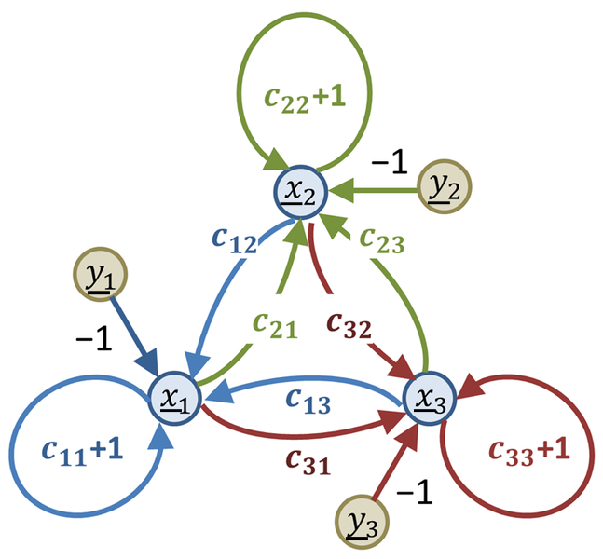
\includegraphics[width=3in]
{control-th/flow_graph_3eqs.png}
\caption{SF graph
that represents a general
system of 3 linear equations 
with 3 unknowns.}
\label{fig-flow-graph-3eqs}
\end{figure}

In Fig.\ref{fig-flow-graph-3eqs},
\beq
\begin{array}{l}
\rvx_1 = (c_{11}+1)\rvx_1 + c_{12}\rvx_2 
+c_{13}\rvx_3 -\rvy_1
\\
\rvx_2 = c_{21}\rvx_1 + (c_{22}+1)x_2
+c_{23}\rvx_3 -\rvy_2
\\
\rvx_3 = c_{31}\rvx_1 + c_{32}\rvx_2
+(c_{33}+1)\rvx_3 -\rvy_3
\end{array}
\eeq
so

\beq
\left[
\begin{array}{c}
\rvy_1
\\
\rvy_2
\\
\rvy_3
\end{array}
\right]
=
\left[
\begin{array}{ccc}
c_{11}&c_{12}&c_{13}
\\
c_{21}&c_{22}&c_{23}
\\
c_{31}&c_{32}&c_{33}
\end{array}
\right]
\left[
\begin{array}{c}
\rvx_1
\\
\rvx_2
\\
\rvx_3
\end{array}
\right]
\eeq
\beq
y=Cx
\eeq
Note that if 
we get rid of the cycles
by setting $c_{11}=c_{22}=c_{33}=-1$,
the {\it general}
system of 3 linear equations 
with 3 unknowns 
cannot be represented.
The cycles are necessary for
doing this.


